%%% Třetí kapitola

\chapter{Testování algoritmu na datech}

V této části shrneme výsledky implementace výpočtu Jonesova polynomu na malých uzlech, náhodých uzlech a na speciálních typech uzlů.
Budeme se zabývat algoritmy A, B a RND, které byly popsány v sekci~\ref{varianty}.

\section{Malé tabulkové uzly}

\begin{figure}[p]\centering
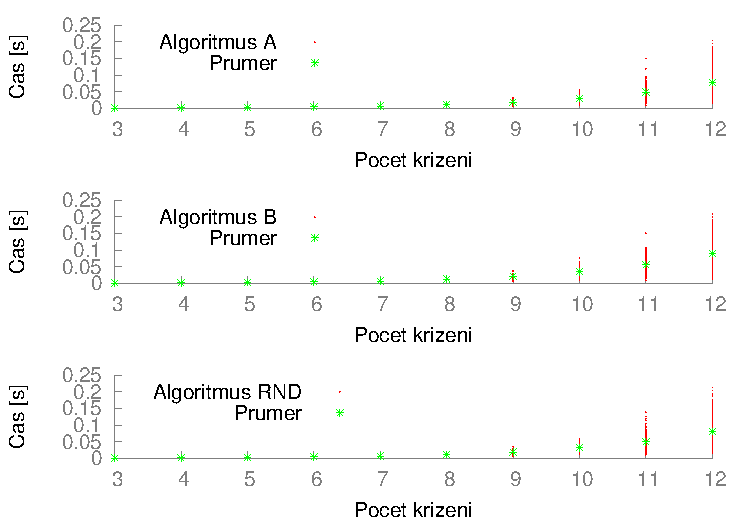
\includegraphics{../img/multiTable}
\caption{Graf dob běhu algoritmů na tabulkových uzlech do 12 křížení s~vyznačenými průměry.}
\label{obr03:multiTable}
\end{figure}

Algoritmy jsme vyzkoušeli na všech uzlech, které mají projekci s maximálně dvanácti kříženími. PD notace uzlů byla získána z databáze KnotInfo~\cite{knotinfo}.
U~všech tří algoritmů byl už u malých uzlů znatelný exponenciální růst doby běhu, viz graf~\ref{obr03:multiTable}. 

Ze srovnání průměrných dob běhu plyne, že nejlepšího času dosahuje algoritmus~A, těsně následuje algoritmus RND a nejpomalejší je algoritmus B, viz~graf~\ref{obr03:srovTable}. 
	
\begin{figure}[p]\centering
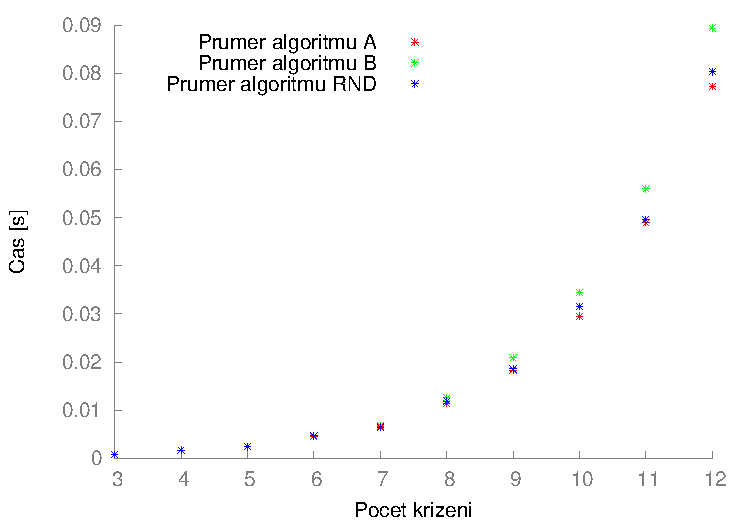
\includegraphics{../img/srovTable}
\caption{Graf průměrných dob běhu algoritmů na tabulkových uzlech do 12~křížení.}
\label{obr03:srovTable}
\end{figure}


\section{Náhodné uzly a linky}

\subsection{Generování náhodných linků a uzlů}
Náhodné linky jsme generovali pomocí rovinných grafů, neboť mezi linky a rovinnými grafy existuje vzájemně jednoznačná korespondence~\cite{Adams2004}. (Jedná se o jinou korespondenci než mezi linky a rovinnými grafy s vrcholy stupně čtyři popsanou v sekci~\ref{jakograf}).

\subsubsection{Převod rovinného grafu na link}
Rovinný graf s $n$ hranami odpovídá linku s $n$ kříženími. Každé hraně přiřadíme náhodně kladné, či záporné znamení a umístíme na ni křížení příslušného typu. Úseky mezi kříženími jsou tím již jednoznačně určené: musí spojovat křížení mezi nejbližšími hranami tak, aby nevznikla žádná další křížení, viz obrázek~\ref{linktriang}.

\subsubsection{Generování náhodných rovinných grafů}
Graf s $n$ hranami získáme následujícím způsobem. Vygenerujeme vhodný počet náhodných bodů v rovině a nalezeneme jejich triangulaci, tj. spojíme body hranami tak, aby byl polygon tvořící konvexní obal bodů rozdělen na trojúhelníky, viz obrázek~\ref{triang}.


\begin{figure}[h]  
\centering 
\begin{subfigure}{0.5\linewidth}\centering
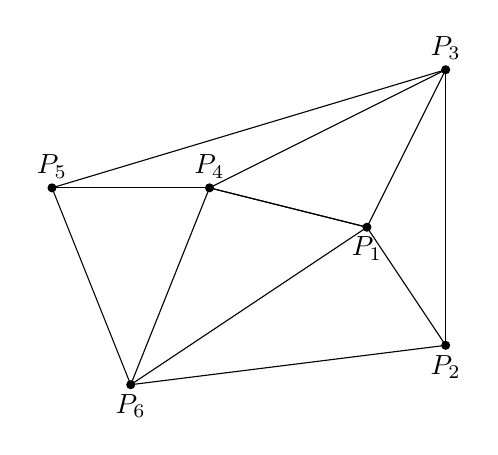
\begin{tikzpicture}
\draw[fill] (1,1) circle [radius=0.05];
\node [below] at (1,1) {$P_1$};

\draw[fill] (2,-1/2) circle [radius=0.05];
\node [below] at (2,-1/2) {$P_2$};

\draw[fill] (2,3) circle [radius=0.05];
\node [above] at (2,3) {$P_3$};

\draw[fill] (-1,3/2) circle [radius=0.05];
\node [above] at (-1,3/2) {$P_4$};

\draw[fill] (-3,3/2) circle [radius=0.05];
\node [above] at (-3,3/2) {$P_5$};

\draw[fill] (-2,-1) circle [radius=0.05];
\node [below] at (-2,-1) {$P_6$};

\draw (-3,3/2) -- (2,3);
\draw (-3,3/2) -- (-1,3/2);
\draw (-3,3/2) -- (-2,-1);
\draw (-1,3/2)  -- (2,3) ;
\draw (-1,3/2)  -- (-2,-1) ;
\draw (-1,3/2)  -- (1,1) ;
\draw (-1,3/2)  -- (1,1) ;
\draw (2,3)   -- (1,1) ;
\draw (-2,-1) -- (1,1) ;
\draw (-2,-1) -- (2,-1/2);
\draw  (1,1)  -- (2,-1/2);
\draw  (2,3)-- (2,-1/2);
\end{tikzpicture}
\caption{Triangulace šesti bodů.} \label{triang}
\end{subfigure}
\begin{subfigure}{0.5\linewidth}\centering
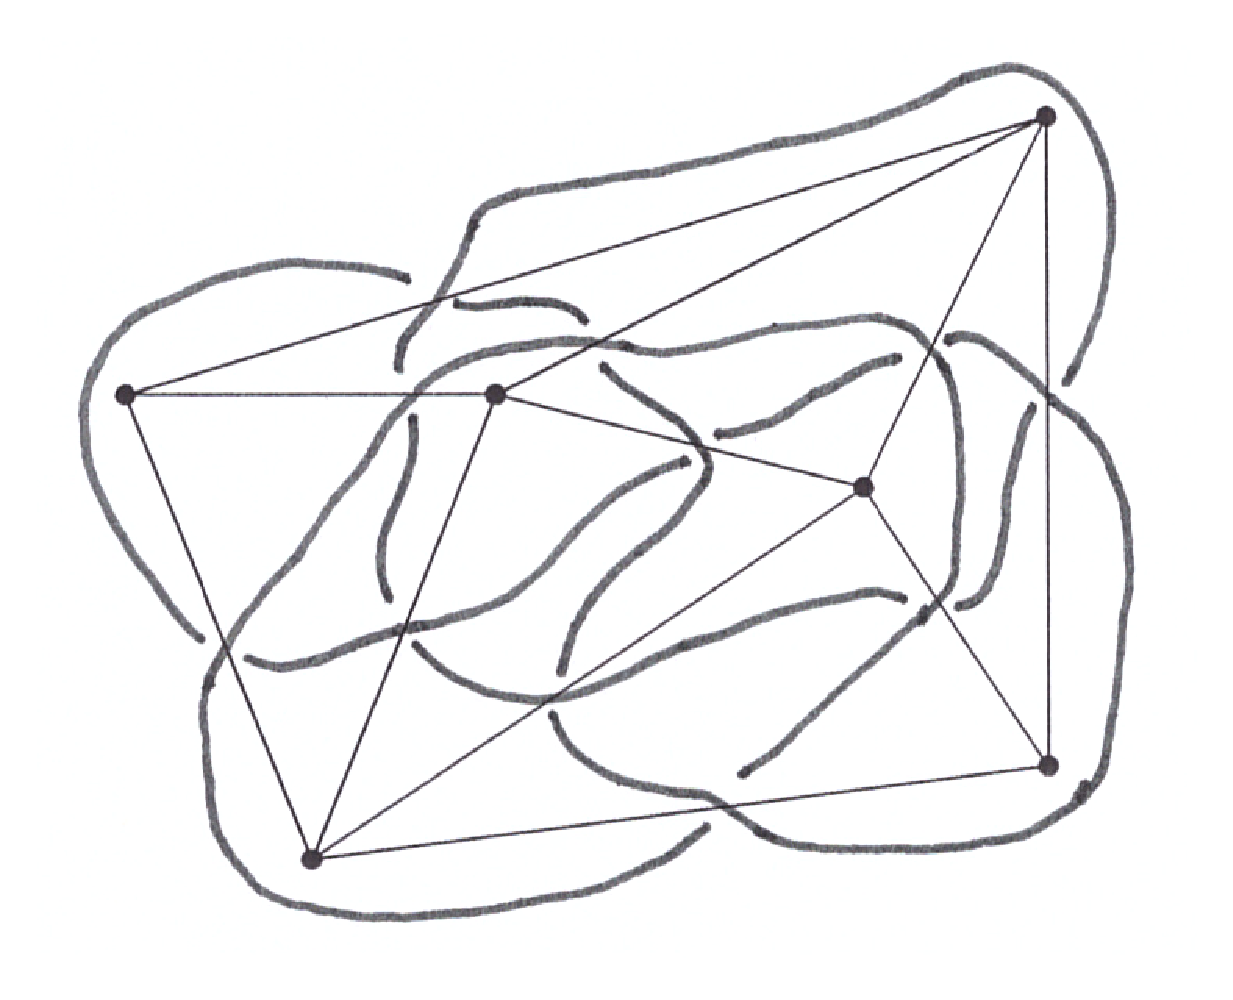
\includegraphics[scale= 0.3]{../img/trianguzel}
\caption{Link vzniklý z triangulace.} \label{linktriang}
\end{subfigure}
\caption{Převod rovinného grafu na link.} 
\end{figure}  


Získali jsme tak rovinný graf s původními body jako vrcholy. Pokud je počet hran menší než $n$, provedeme triangulaci znovu s větším počtem bodů. Pokud je počet hran větší než $n$, odstraníme potřebný počet náhodně zvolených hran.


\subsubsection{Implementace}

Triangulace bodů je snadno implementovatelný geometrický problém. 

Se získaným rovinným grafem pracujeme jako s množinou vrcholů a k nim příslušným hranám. Hrany jsou seřazeny podle pořadí, jak k danému vrcholu v~nakreslení grafu přiléhají. Z této struktury je již možné získat PD notaci příslušného linku.


V PD notaci lze procházkou po vláknu snadno poznat, jestli je vygenerovaný link uzlem. Také jsme jednoduchou operací schopni uzel změnit na alternující, tedy takový, v němž se střídají křížení vedená zdola a svrchu.

Dokážeme tedy nagenerovat uzly, alternující uzly a linky libovolné velikosti.

Takto generované uzly jsou většinou buď rozmotané, nebo lze rozmotáním odstranit pouze několik křížení.

\subsection{Test}

\begin{figure}[p]\centering
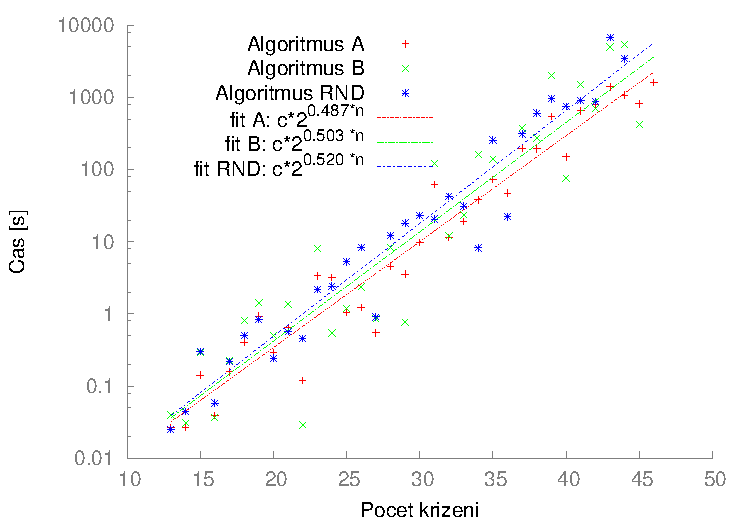
\includegraphics{../img/knotsFIT}
\caption{Graf dob běhu algoritmů na náhodných uzlech proložené křivkami, logaritmická škála.}
\label{obr03:knotSrov}
\end{figure}

\begin{figure}[p]\centering
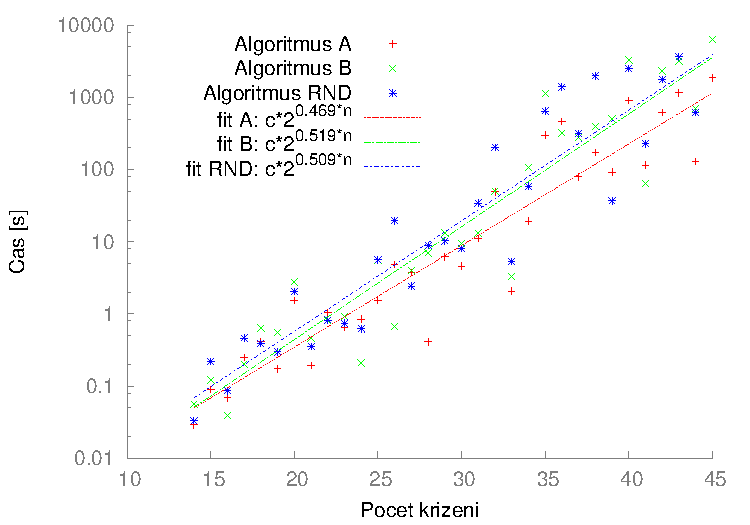
\includegraphics{../img/alt_knotsFIT}
\caption{Graf dob běhu algoritmů na náhodných alternujících uzlech proložené křivkami, logaritmická škála.}
\label{obr03:altSrov}
\end{figure}

\begin{figure}[p]\centering
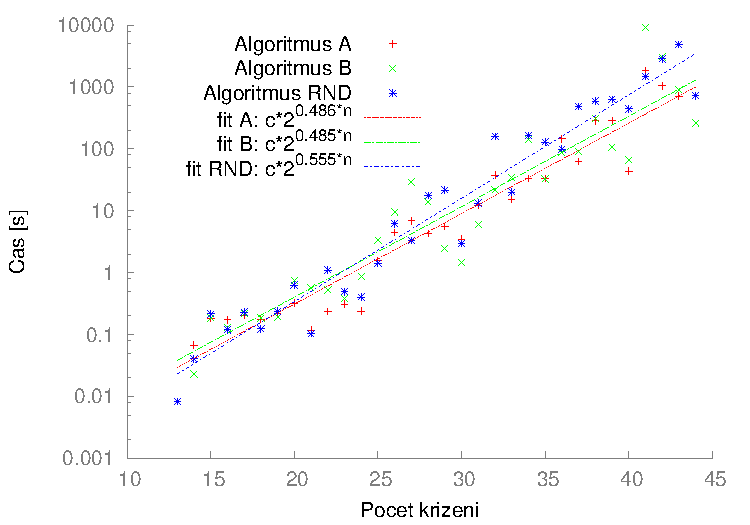
\includegraphics{../img/linksFIT}
\caption{Graf dob běhu algoritmů na náhodných lincích proložené křivkami, logaritmická škála.}
\label{obr03:linkSrov}
\end{figure}


\begin{table}[p]
\centering
  \begin{tabular}{*{8}{c}}
    \toprule
       & A & chyba A & B & chyba B &  RND & chyba RND \\ 
    \midrule
    Uzly  & 0,487 & $\pm$ 0,020  &   0,503 & $\pm$ 0,036   &  0,520 & $\pm$ 0,024\\
    Alternující uzly & 0,468  & $\pm$ 0,030 &  0,519 & $\pm$  0,033 & 0,509 & $\pm$ 0,036\\
    Linky  & 0,486 &  $\pm$ 0,024 &   0,485 & $\pm$  0,032  &   0,555 & $\pm$ 0,024\\
    \bottomrule
  \end{tabular}
    \caption{Odhady koeficientu $k$ průměrné časové složitosti $\mathcal{O}\left(2^{kn + o(n)}\right)$ jednotlivých algoritmů podle druhu dat.} \label{datatab}

\end{table} 

Rychlost algoritmů jsme otestovali na uzlech (graf~\ref{obr03:knotSrov}), alternujících uzlech (graf~\ref{obr03:altSrov}) a lincích (graf~\ref{obr03:linkSrov}) s počtem křížení $n \leq 46$. 

Pokusíme se u jednotlivých algoritmů v závislosti na druhu testovaných dat odhadnout průměrnou časovou složitost $T(n)$. Na základě odhadů složitosti dokázaných v sekci~\ref{analyza} budeme předpokládat, že $T(n) = \mathcal{O} \left(2^{kn + o(n)}\right)$ pro jistý koeficient $k$.

Označme $t(n) = \log_2(T(n)) = \mathcal{O} \left(kn + o(n)\right) $. Sublineární členy nahradíme konstantou a odhad koeficientu $k$ získáme lineární regresí logaritmu naměřených dat, viz tabulka~\ref{datatab}.

Podle výsledků Jonesův polynom nejrychleji počítá algoritmus A, který volí křížení ve stěně ohraničené dvěma hranami. Odhad jeho průměrné časové složitosti na uzlech a lincích je $\mathcal{O}\left(2^{0,49n+ o(n)}\right)$, na alternujících uzlech $\mathcal{O}\left(2^{0.468 n+ o(n)}\right)$. Volba tohoto křížení tedy v průměru vede k většímu rozmotávání než volba křížení ve stěně typu B nebo náhodná volba křížení. 

Algoritmus B dosahuje různých výsledků v závislosti na druhu dat. Na lincích má podobnou průměrnou časovou složitost jako algoritmus A, ovšem na alternujících uzlech odhaduje jeho průměrnou složitost $\mathcal{O}\left(2^{0,519 n+ o(n)}\right)$, což je ze všech variant nejvíce. Odpovídá to i výsledku testování na tabulkových uzlech, kde byl tento algoritmus také nejpomalejší, neboť uzel bývá zaznamenán v alternujícím nakreslení, pokud takové nakreslení existuje. Ačkoli tedy algoritmus B zaručuje ze všech algoritmů u synů největší rozmotání, viz sekce~\ref{steny}, může na určitých datech běžet nejpomaleji. Na obecných uzlech ovšem dostáváme podobný odhad průměrné složitosti jako u algoritmu A.

Také výsledky algoritmu RND se liší podle druhu testovaných dat. Nejlépe se mu daří na alternujících uzlech, u nichž průměrnou složitost odhadujeme $\mathcal{O}\left(2^{0,509 n+ o(n)}\right)$. Naopak nejpomalejší je na lincích s odhadem $\mathcal{O}\left(2^{0,555 n+ o(n)}\right)$. Náhodná volba křížení pravděpodobně vede k rozpadání na disjuntkní uzly, což prodlužuje výpočet.

Odhad koeficientu $k$ se často pohybuje kolem hodnoty $k=0,5$. Složitost $\mathcal{O}\left(2^{0,5 n}\right)$ odpovídá průběhu algoritmu, v němž dojde u každého syna k rozmotání právě jednoho křížení. Platila by tedy rekurence
$$T(n) = 2T(n-2).$$




\section{Torusové uzly} \label{torus}



Rychlost algoritmů jsme vyzkoušeli na 36 nejmenších torusových uzlech. Jejich PD notaci jsme získali z databáze Knot Atlas~\cite{knotatlas}.

Na grafu dob běhu algoritmů lze rozlišit dva shluky bodů, viz graf~\ref{obr03:torusSrov}. Spodní shluk odpovídá torusovým uzlům ($2k+1$, 2), tedy těm, které se obmotají dvakrát podél osy rotace torusu a jejich diagram má tvar dvou zakroucených vláken s~$2k+1$ kříženími.

\begin{figure}[H]\centering
\begin{tikzpicture}[use Hobby shortcut, scale=0.75]
\begin{knot}[
  consider self intersections=true,
%  draft mode=crossings,
  flip crossing/.list={2,4,6} 
]
\strand ([closed]90:2) foreach \k in {1,...,7} { .. (90-360/7+\k*720/7:1.5) .. (90+\k*720/7:2) } (90:2);
\end{knot}
\end{tikzpicture}
\caption{Torusový uzel (7,2).}
\label{obr03:torus7}
\end{figure}

\begin{figure}[p]\centering
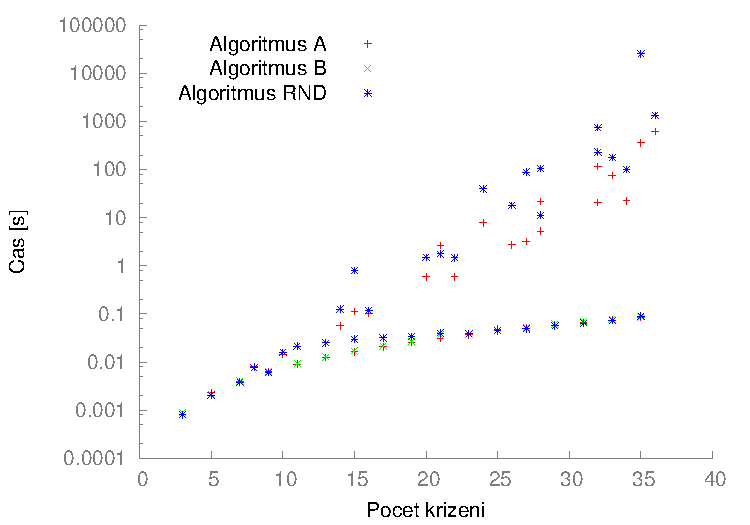
\includegraphics{../img/torusSrov}
\caption{Graf dob běhu algoritmů na 36 torusových uzlech, logaritmická škála.}
\label{obr03:torusSrov}
\end{figure}

\begin{figure}[b]\centering
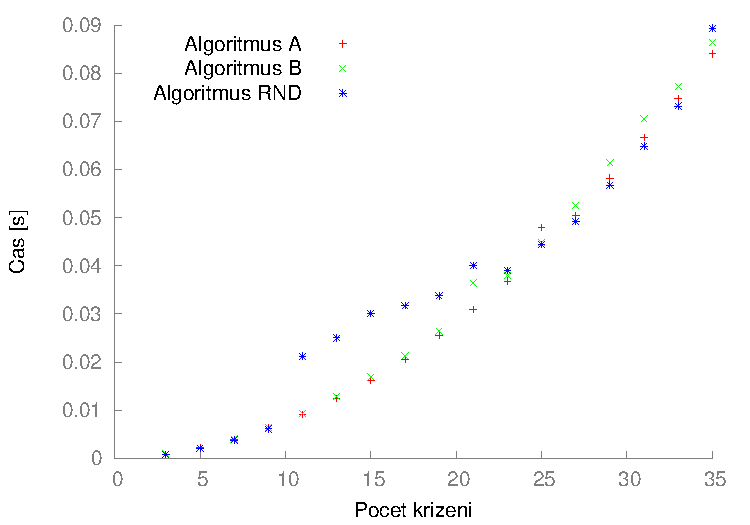
\includegraphics{../img/torus2}
\caption{Doby běhu algoritmů na torusových uzlech (3,2) až (35,2).}
\label{obr03:torus2}
\end{figure}

Všechny stěny těchto uzlů jsou ohraničené pouze dvěma hranami. Rozpojením libovolného křížení jedním směrem vznikne torusový link ($2k$, 2), druhým směrem triviální uzel, který lze rozmotat několika prvními Reidemeistrovými pohyby. Z~linku zase rozpojením libovolného křížení vznikne uzel ($2k-1$, 2). Rozpojení a rozmotávání má lineární časovou složitost, celkově tedy všechny tři algoritmy spočítají Jonesův polynom tohoto typu torusových uzlů v kvadratickém čase, což lze pozorovat na grafu~\ref{obr03:torus2}.

\begin{figure}[p]\centering
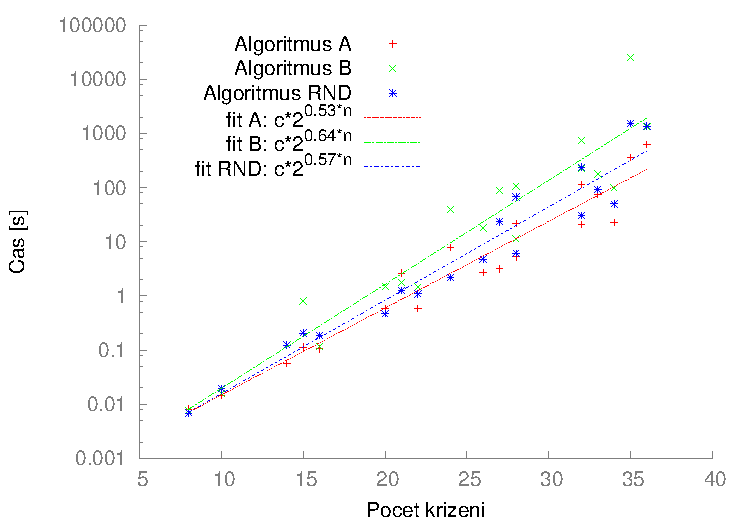
\includegraphics{../img/torusNe2FIT}
\caption{Doby běhu algoritmů na malých torusových uzlech ($p$, $q\neq 2$) proložené křivkami, logaritmická škála.}
\label{obr03:torusFIT}
\end{figure}

Na torusových uzlech tvaru ($p$, $q$), kde $q\neq 2$ již doba běhu algoritmu roste exponenciálně, viz graf~\ref{obr03:torusFIT}). Opět jsme provedli odhad průměrných časových složitostí, viz tabulka~\ref{torustab}.

\begin{table}[t]
\centering
  \begin{tabular}{*{8}{c}}
    \toprule
       & A & chyba A & B & chyba B &  RND & chyba RND \\ 
    \midrule
      & 0,533 & $\pm$ 0,032  &   0,638 & $\pm$ 0,048   &  0,572 & $\pm$ 0,035\\
    \bottomrule
  \end{tabular}
    \caption{Odhady koeficientu $k$ průměrné časové složitosti $\mathcal{O}\left(2^{kn} + o(n)\right)$ jednotlivých algoritmů na typu torusových uzlů ($p$, $q\neq 2$) .} \label{torustab}
    
\end{table}

Všechny varianty algoritmů jsou na torusových uzlích pomalejší než na náhodných datech. Nejrychlejší je opět algoritmus A s průměrnou časovou složitostí $\mathcal{O}\left(2^{0,533 n + o(n)}\right)$. Naopak nejpomalejší je algoritmus B se složitostí $\mathcal{O}\left(2^{0,638 n + o(n)}\right)$, což je nejvyšší složitost, kterou jsme při testování získali.
